%%%%%%%%%%%%%%%%%%%%%%%%%%%%%%%%%%%%%%%%%%%%%%%%%%%%%%%%%%%%%%%%%%%%%%%%%%%%%%%%
%%%%%%%%%%%%%%%%%%   Vorlage für eine Abschlussarbeit   %%%%%%%%%%%%%%%%%%%%%%%%
%%%%%%%%%%%%%%%%%%%%%%%%%%%%%%%%%%%%%%%%%%%%%%%%%%%%%%%%%%%%%%%%%%%%%%%%%%%%%%%%

% Erstellt von Maximilian Nöthe, <maximilian.noethe@tu-dortmund.de>
% ausgelegt für lualatex und Biblatex mit biber

% Kompilieren mit
% latexmk --lualatex --output-directory=build thesis.tex
% oder einfach mit:
% make

\documentclass[
  tucolor,       % remove for less green,
  BCOR=12mm,     % 12mm binding corrections, adjust to fit your binding
  parskip=half,  % new paragraphs start with half line vertical space
  open=any,      % chapters start on both odd and even pages
  cleardoublepage=plain,  % no header/footer on blank pages
]{tudothesis}


% Warning, if another latex run is needed
\usepackage[aux]{rerunfilecheck}

% just list chapters and sections in the toc, not subsections or smaller
\setcounter{tocdepth}{1}

%------------------------------------------------------------------------------
%------------------------------ Fonts, Unicode, Language ----------------------
%------------------------------------------------------------------------------
\usepackage{fontspec}
\defaultfontfeatures{Ligatures=TeX}  % -- becomes en-dash etc.

% load english (for abstract) and ngerman language
% the main language has to come last
\usepackage[american]{babel}

% intelligent quotation marks, language and nesting sensitive
\usepackage[autostyle]{csquotes}

% microtypographical features, makes the text look nicer on the small scale
\usepackage{microtype}

%------------------------------------------------------------------------------
%------------------------ Math Packages and settings --------------------------
%------------------------------------------------------------------------------

\usepackage{amsmath}
\usepackage{amssymb}
\usepackage{mathtools}

% Enable Unicode-Math and follow the ISO-Standards for typesetting math
\usepackage[
  math-style=ISO,
  bold-style=ISO,
  sans-style=italic,
  nabla=upright,
  partial=upright,
  warnings-off={mathtools-colon,mathtools-overbracket}, % suppress some unnecessary warnings
]{unicode-math}
\setmathfont{Latin Modern Math}

% nice, small fracs for the text with \sfrac{}{}
\usepackage{xfrac}


%------------------------------------------------------------------------------
%---------------------------- Numbers and Units -------------------------------
%------------------------------------------------------------------------------

\usepackage[
  locale=DE,
  separate-uncertainty=true,
  per-mode=symbol-or-fraction,
]{siunitx}

%------------------------------------------------------------------------------
%-------------------------------- tables  -------------------------------------
%------------------------------------------------------------------------------

\usepackage{booktabs}       % \toprule, \midrule, \bottomrule, etc

%------------------------------------------------------------------------------
%-------------------------------- graphics -------------------------------------
%------------------------------------------------------------------------------

\usepackage{graphicx}
% currently broken
% \usepackage{grffile}

% allow figures to be placed in the running text by default:
\usepackage{scrhack}
\usepackage{float}
\floatplacement{figure}{htbp}
\floatplacement{table}{htbp}

% keep figures and tables in the section
\usepackage[section, below]{placeins}

% allows to include PDFs as full pages
\usepackage{pdfpages}

% Set the PDF Version of this document to 1.7 (1.4 is the current default)
% This is needed so that PDFs with Version >1.5 can be included
\pdfvariable minorversion=7

%------------------------------------------------------------------------------
%---------------------- customize list environments ---------------------------
%------------------------------------------------------------------------------

\usepackage{enumitem}

%------------------------------------------------------------------------------
%------------------------------ Bibliographie ---------------------------------
%------------------------------------------------------------------------------

\usepackage[
  backend=biber,   % use modern biber backend
  autolang=hyphen, % load hyphenation rules for if language of bibentry is not
                   % german, has to be loaded with \setotherlanguages
                   % in the references.bib use langid={en} for english sources
]{biblatex}
\addbibresource{references.bib}  % the bib file to use
\DefineBibliographyStrings{german}{andothers = {{et\,al\adddot}}}  % replace u.a. with et al.


% Last packages, do not change order or insert new packages after these ones
\usepackage[pdfusetitle, unicode, linkbordercolor=tugreen, citebordercolor=tugreen]{hyperref}
\usepackage{bookmark}
\usepackage[shortcuts]{extdash}
\usepackage{makecell}

%------------------------------------------------------------------------------
%-------------------------    Angaben zur Arbeit   ----------------------------
%------------------------------------------------------------------------------

\author{Sebastian Fischer}
\title{Analyzing Coincident Muon events in the IceCube Neutrino Observatory with a focus on the Fixed Rate Trigger}
\date{2025}
\birthplace{Göttingen}
\chair{Arbeitsgruppe Astroteilchenphysik}
\division{Fakultät Physik}
\thesisclass{Bachelor of Science}
\submissiondate{25.01.2025}
\firstcorrector{Prof.~Dr.~Dr. Wolfgang Rhode}
\secondcorrector{Dr. Jens Weingarten}

% tu logo on top of the titlepage
\titlehead{\includegraphics[height=1.5cm]{logos/tu-logo.pdf}}

\begin{document}
\frontmatter
% \thispagestyle{empty}
% \setcounter{page}{2}
% \section*{Hinweise}
% Empfohlen wird die Verwendung dieser Vorlage mit der jeweils aktuellsten TeXLive Version (Linux, Windows) bzw. MacTeX Version (MacOS).
% Aktuell ist dies TeXLive 2021. Download hier:
% \begin{center}
%   \ttfamily\url{https://www.tug.org/texlive/}
% \end{center}

% Die Vorlage \texttt{thesis.tex} ist für die Kompilierung mit \texttt{lualatex} ausgelegt, mit wenigen Anpassungen kann sie aber auch mit \texttt{pdflatex} oder \texttt{xelatex} verwendet werden.
% Die Dokumentenklasse \texttt{tudothesis.cls} kann mit allen drei Programmen verwednet werden.

% Achten Sie auch auf die Kodierung der Quelldateien.
% Bei Verwendung von Xe\LaTeX\ oder Lua\LaTeX\ (empfohlen) müssen die
% Quelldateien UTF-8 kodiert sein.
% Bei Verwendung von pdf\LaTeX\ nutzen Sie die Pakete \texttt{inputenc} und \texttt{fontenc} mit der korrekten Wahl der Kodierungen.

% Eine aktuelle Version dieser Vorlage steht unter 
% \begin{center}
%   \ttfamily\url{https://github.com/maxnoe/tudothesis}
% \end{center}
% zur Verfügung.

% Alle verwendeten Pakete werden im \LaTeX{} Kurs von Pep et al.\ erklärt:
% \begin{center}
%   \ttfamily\url{http://toolbox.pep-dortmund.org/notes}
% \end{center}

% Für Rückmeldungen und bei Problemen mit der Klasse oder Vorlage, bitte ein \emph{Issue} auf GitHub aufmachen oder eine Email an
% \href{mailto:maximilian.noethe@tu-dortmund.de}{maximilian.noethe@tu-dortmund.de} schreiben.

% Wenn Sie die Dokumentenklasse mit der Option \texttt{tucolor} laden, werden verschiedene Elemente in TU-Grün gesetzt.

\maketitle

% Gutachterseite
\makecorrectorpage

% hier beginnt der Vorspann, nummeriert in römischen Zahlen
% \thispagestyle{plain}

% \section*{Kurzfassung}
% Hier steht eine Kurzfassung der Arbeit in deutscher Sprache inklusive der Zusammenfassung der
% Ergebnisse.
% Zusammen mit der englischen Zusammenfassung muss sie auf diese Seite passen.

% \section*{Abstract}
% \begin{foreignlanguage}{english}
% The abstract is a short summary of the thesis in English, together with the German summary it has to fit on this page.
% \end{foreignlanguage}

\tableofcontents

\mainmatter
% Hier beginnt der Inhalt mit Seite 1 in arabischen Ziffern
% \thispagestyle{plain}

% \section*{Kurzfassung}
% Hier steht eine Kurzfassung der Arbeit in deutscher Sprache inklusive der Zusammenfassung der
% Ergebnisse.
% Zusammen mit der englischen Zusammenfassung muss sie auf diese Seite passen.

% \section*{Abstract}
% \begin{foreignlanguage}{english}
% The abstract is a short summary of the thesis in English, together with the German summary it has to fit on this page.
% \end{foreignlanguage}

\chapter{Introduction}

The IceCube Neutrino Observatory, located at the geographic South Pole, is the largest particle detector of its kind, designed to detect high-energy neutrinos originating 
from astrophysical sources. One of the challenges in IceCube's data analysis lies in identifying coincident muon events, which occur when two or more muons or muon bundles
from separate 
primary particles reach the detector within a short time window. Understanding these events provides valuable insights into cosmic ray interactions and the 
detector's capabilities.
This thesis focuses on analyzing coincident events in IceCube with a particular emphasis on the Fixed Rate Trigger (FRT), a unique data acquisition method that 
records unfiltered signals across the entire detector. Unlike other triggers that apply stringent filtering criteria, the FRT provides a comprehensive view of 
unfiltered signals, making it ideal for studying coincident events. However, the lack of easily measurable differences between signals and noise poses challenges 
in distinguishing significant signals from background noise.
To address this, a combination of theoretical modeling and data analysis was employed. Theoretical calculations based on Poisson statistics were used to estimate 
coincidence rates, while a Python-based peak detection algorithm was applied to identify significant subevents within FRT data. 
This thesis is structured as follows: Chapter~\ref{chap:theory} provides the theoretical background, including an overview of the IceCube detector, the physics of Cherenkov 
radiation, and the concept of coincident events. Chapter~\ref{chap:results} presents the results of the analysis, including the theoretical estimation of coincidence probabilities 
and the analysis of FRT data. The concluding discussion highlights the broader implications of the findings and potential directions for future research.

\chapter{Theory}\label{chap:theory}
% Hier folgt eine kurze Einleitung in die Thematik der Bachelorarbeit.
% Die Einleitung muss kurz sein, damit die vorgegebene Gesamtlänge der 
% Arbeit von 25 Seiten nicht überschritten wird. 
% Die Beschränkung der Seitenzahl sollte man ernst nehmen,
% da Überschreitung zu Abzügen in der Note führen kann. 
% Um der Längenbeschränkung zu genügen, darf auch nicht an der Schriftgröße,
% dem Zeilenabstand oder dem Satzspiegel (bedruckte Fläche der Seite) manipuliert werden.

\section{A General Overview of the IceCube Detector}
The IceCube neutrino detector is a cubic kilometer scale particle detector located near the Amundsen-Scott South Pole Station. The primary goal of 
the detector is the detection of high energy neutrinos as messenger particles for the study of astrophysical sources. The detector unit is split into three 
parts, which are the In-Ice/IceTop, and DeepCore arrays. 

In-Ice is the largest component and consists of 86 vertical strings, extending vertically into the ice below the surface for \SI{2450}{\metre}. 
Each of the strings contains 60 Digital Optical Modules (DOMs) starting from a depth of \SI{1450}{\metre} all the way down to \SI{2450}{\metre}
The DOMs are evenly separated by \SI{17}{\metre} alongside their respective string, making a total number of \num{5160} DOMs. 

IceTop, as the name suggests, is located at the surface of the ice with \num{162} tanks filled with ice and equipped with PMTs. 
The tanks are arranged in 81 stations in a manner that approximately mimics the structure of the In-Ice Array. 

DeepCore, a sub-array within the In-Ice Array, is located below \SI{1750}{\metre}. It contains an extra \num{8} strings alongside the 
\num{7} strings from the In-Ice Array. This creates a more densly packed arrangement of DOMs in the lower center of the detector, which increases its 
ability to detect low-energy signals. 

Figure~\ref{fig:icecube_sketch_01} shows a visual representation of this structure. For more details on the structure and build of the detector, see \cite{Aartsen_2017}.

\begin{figure}[htbp]
    \centering
    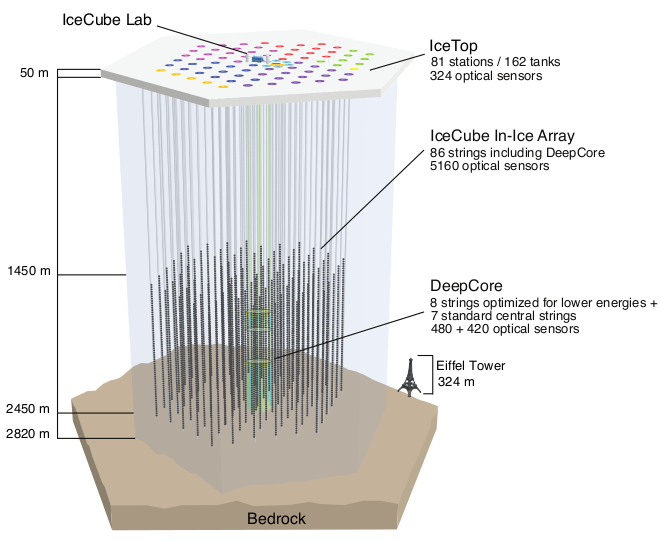
\includegraphics[width=0.7\textwidth]{content/pictures/icecube_sketch_01.png}
    \caption{An overview of the arrangement inside of the detector.\cite{Aartsen_2017}}\label{fig:icecube_sketch_01}
\end{figure}

\section{Digital Optical Module}\label{sec:dom}

A single DOM consists of a glass housing, containing the PMT and the corresponding circuit boards. The technical part of the functionality of 
the circuit boards are not of interest for this analysis, so I will not go into detail on that topic. The PMT however is the actual detecting unit of 
the DOM~. A sketch of a PMT is shown in figure~\ref{fig:pmt01}.

\begin{figure}[htbp]
    \centering
    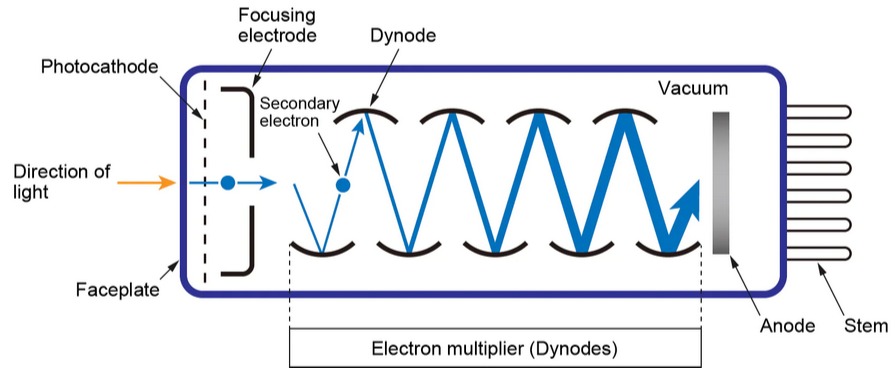
\includegraphics[width=\textwidth]{content/pictures/pmt_sketch_01.png}
    \caption{The Principle Construction of a Photomultiplier\cite{photomultiplier_matsusada}.}\label{fig:pmt01}
\end{figure}

When a photon with sufficient energy hits the photocathode of the PMT, its energy is absorbed and an electron is emitted via the photoelectric effect.
The electron is accelerated towards the first dynode due to its electric charge. Hitting the dynode triggers secondary emissions, increasing the total 
number of electrons emitted. This process repeats itself for the number of dynodes the PMT comprises. After the final amplification by the last 
dynode the electrons are collected by the anode, which produces a current proportional to the intensity of the initial light signal, meaning the amount of
photons hitting the PMT\@. 

\section{Cherenkov Radiation}

The light detected by the photomultipliers is only a secondary signal called Cherenkov radiation~\cite{PhysRevX.13.011002}. It is created when a charged particle travels through a 
dielectric medium with a velocity greater than the speed of light inside of this medium. The charged particle polarizes the medium's molecules in its
immediate surroundings as it passes through. The excited molecules then return to their ground state by emitting their superfluous energy as light.
Because the light travels slower than the particle exciting the molecules, the light waves do not interfere destructively, but form a conical shock front, similar to that of an object moving through air at supersonic velocities. This cone of light is the Cherenkov radiation detected by the PMTs.
As explained in section~\ref{sec:dom}, the measured charge is proportional to the intensity of the Cherenkov radiation, which itself is proportional to the 
energy lost by the particle inducing the radiation. Another important value is the angle of the cherenkov light cone, which is dependent on the velocity of the 
particle creating it. This relation is given by 
\begin{equation}
    \cos{\theta_c} = \frac{c}{nv},
\end{equation}
where $n$ is the refractive index of the medium. A higher velocity will therefore lead to a larger angle and vice versa, which, together with the information about 
the charge deposited in the DOMs, enables the possibility of recreating the detected particle's characteristics.

\section{Muons}\label{sec:muons}

A significant proportion of the particles measured in IceCube are muons, which are elementary particles categorized as leptons by the standard model.
This means they carry an electric charge of $\pm 1e$ and have spin $\frac{1}{2}$. The mass of the muon is \num{105.658}\text{MeV}. IceCube detects
muons at a rate of roughly \SI{2500}{Hz}. When cosmic rays collide with the atmosphere's molecules, a multitude of secondary particles are created including 
pions and kaons. The average lifetime of these mesons are of the magnitude of \SI{e-8}{s} or less. Their resulting decay products include muons which are 
produced via the following decay modes:\\

\begin{align}
    \pi^\pm \to \mu^\pm + \nu_\mu \\
    K^\pm \to \mu^\pm + \nu_\mu
\end{align}

These muons have an average lifetime of about \SI{2.2}{\micro\second}, which allows a significant fraction of them to reach the Earths surface due to their 
ultrarelativistic velocities. Details on the effects of relativistic velocities on spacetime can be found in~\cite{deBarros2016}. When a muon travels through the ice 
within the IceCube detector, it produces Cherenkov radiation due to its charge and high velocities and 
can thus be indirectly measured. Realistically, muons which hit the detector are usually clustered up in bundles, since the cosmic rays responsible for their production
mostly create multiple secondary particles which then decay into muons. Analyzing the cumulative energies of these bundles can provide some insight into the primary 
energies of the original cosmic rays. For a deeper look into the physical characteristics of muons and their creation in the atmosphere, see~\cite{Cecchini2012}.


\section{Data Acquisition}\label{sec:daq}

A single DOM measureing a signal is not able to distinguish between different types of events, since its only capability lies in the detection of a current
caused by photons hitting the PMT\@. In order to distinguish between noise and possible signals stemming from Cherenkov radiation, multiple requirements are
put in place to ensure that the full data of a signal is only saved for those signals that might constitute a real event. The data acquisition systems (DAQ)
is the software complex responsible for filtering signals by different characteristics. The first step for any signal is to scan for so called hard local 
coincidences (HLC). This condition is met when there are multiple hits registered in neighbouring DOMs within a certain time frame.
There are \textit{triggers} implemented which search for multiplicities of HLC hits within a certain time frame and with certain spatial requirements.
The specific requirements for different triggers are given in table~\ref{tab:trigger_config}.
The simplest one is the simple multiplicity trigger (SMT), which triggers whenever at least $N$ HLC hits occur within a time frame of some 
\si{\micro\second}. This sets a set of intuitive conditions for grouping a cluster of signals into an event that could be a muon or another 
charged particle emitting Cherenkov radiation. \\
The Fixed Rate Trigger (FRT), a key focus of this thesis, operates differently from other triggers as it does not rely on any signal multiplicity. Instead, it is
a time-based trigger that reads out the entire detector—capturing data from all operational DOMs—for a duration of \SI{10}{ms} every \SI{300}{s}. With no additional
selection criteria, the FRT records all detected signals during the readout period.

The FRT thus opens a window into the unfiltered distribution of signals collected by the detector. Since the FRT data undergoes no reduction, 
it includes both background noise and low-energy signals. Due to its comparatively long readout window, the signals captured within a single 
FRT event are split into multiple subevents through an automated process. On a temporal scale, these subevents represent distinct intervals within the event 
where significant signals are detected. 
Hypothetically, if the diagnoses of relevant subevents happens flawlessly, filtering out 
the subevents would yield a clear picture of the noise distribution in IceCube. 



\begin{table}[htbp]
    \vspace{0.5cm}
    \centering
    \caption{Trigger configurations and their parameters\cite{Aartsen_2017}.}
    \renewcommand{\arraystretch}{1.3} % Adjust row height for better spacing
    \setlength{\tabcolsep}{6pt} % Adjust column spacing for better alignment
    \resizebox{\textwidth}{!}{
    \begin{tabular}{@{}llclcl@{}}
    \toprule
    \textbf{Trigger} & \textbf{DOM set}    & \textbf{\(N\) HLC hits} & \textbf{Window (\(\mu s\))} & \textbf{Topology} & \textbf{Rate (Hz)} \\ \midrule
    SMT              & in-ice              & 8                       & 5                          & ---               & 2100               \\
    SMT              & DeepCore            & 3                       & 2.5                        & ---               & 250                \\
    SMT              & IceTop              & 6                       & 5                          & ---               & 25                 \\
    Volume           & in-ice              & 4                       & 1                          & cylinder (\(r=175\,\mathrm{m}, h=75\,\mathrm{m}\)) & 3700               \\
    Volume           & IceTop infill       & 4                       & 0.2                        & cylinder (\(r=60\,\mathrm{m}, h=10\,\mathrm{m}\))  & 4                  \\
    String           & in-ice              & 5                       & 1.5                        & 7 adjacent vertical DOMs                    & 2200               \\
    SLOP             & in-ice              & \(N_{\text{triplet}}=5\) & \(\begin{array}{l} T_{\text{prox}}=2.5,\\ T_{\min}=0,\\ T_{\max}=500 \end{array}\) & \(\begin{array}{l} \alpha_{\min}=140^\circ, v_{\text{rel}}^{\max}=0.5\end{array}\) & 12 \\
    FRT              & all                 & ---                     & ---                        & ---               & 0.003              \\ \bottomrule
    \end{tabular}}
    \label{tab:trigger_config}
\end{table}

% \begin{figure}[htbp]
%     \centering
%     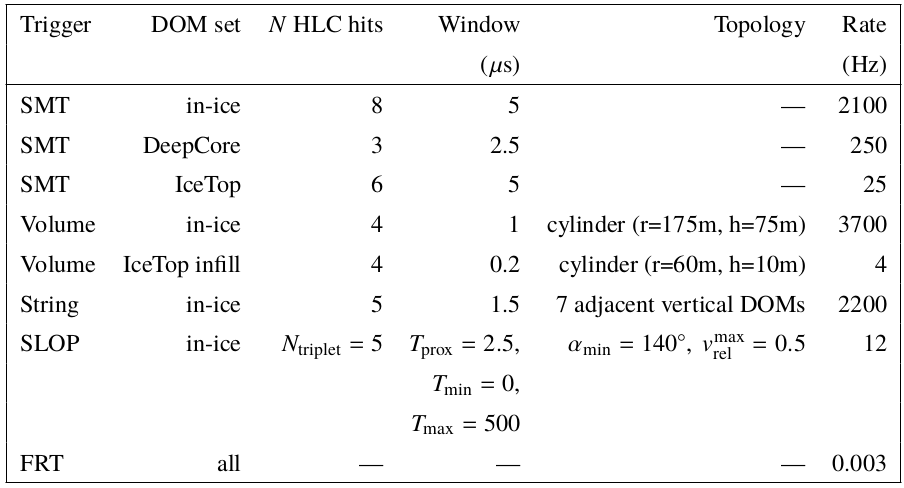
\includegraphics[width=\textwidth]{content/pictures/trigger_list.png}
%     \caption{A list of all triggers in IceCube.}\label{fig:triggers}
% \end{figure}

\section{Coincident Events}\label{sec:coin}

The primary goal of this thesis is the analysis of coincident events in IceCube. This is not to be confused with coincident signals or hits, which are used 
to determine if indeed an event is constituted by the signals. A coincident event however means that two or more muons or muon bundles from different primary 
particles hit the detector within the 
time frame of a readout window from a certain trigger. The SMT for example will group together any multiplicity of HLC hits in the detector and categorize them as one
event, as long as no other measures are taken. If there are multiple muon bundles resulting from different primary particles, the resulting compound signal would be
forwarded as one event. The information about the reality, that the measured signal consists of two different primary particles, would be lost. \\
Firstly, an estimation can be made about the percentile of coincident events for any given event rate. As a generic model correction of event rate and 
coincident event rate, a Poisson distribution is a sensible approach, as explained in detail in~\cite{Ellis2019}. 

\begin{equation}
    P_{\lambda}(k) = \frac{\lambda^k}{k!}\text{e}^{-\lambda} \; .
\end{equation}

$\lambda$ is the expected value, which can be rewritten as 

\begin{equation}
    \lambda = R \cdot \tau \; ,
\end{equation}

where $R$ is the rate of incoming particles and $\tau$ is the search time frame set by the trigger, as explained in section\.~\ref{sec:daq}. 
The value of interest is the probability for 2 or more particles hitting the detector within a certain time frame. This yields \\

\begin{equation}
    P_{\lambda = R\cdot\tau}(k\geq2) = e^{- R\cdot\tau} \cdot \sum_{k=2}^\infty \frac{{(R\cdot\tau)}^k}{k!} \; .
\end{equation} 

Multiplying with the event rate $R$ then yields the coincidence rate $R_{co}$ depending on the event rate and the readout window $\tau$:

\begin{equation}
    R_{co}(R,\tau) = R \cdot e^{- R\cdot\tau} \cdot \sum_{k=2}^\infty \frac{{(R\cdot\tau)}^k}{k!}\;.
    \label{eq:multi_rate}
\end{equation}

This makes for a useful connection between the coincidence event rate and any spectrum that has a known or easily producible relation to a certain event rate.

% \section{Different spectrums for visualizations}\label{sec:sp

% % energy spectrum and zenith angle spectrum ? 
% The majority of graphics shown in the analysis part of this thesis, are some variables of interest on either one of the following spectrums. I will thus briefly 
% explain the theory behind their physical meanings in the context of the IceCube detector. 

% \subsection{The Energy Spectrum}
% Energy as a direct observable in IceCube is not something one has access to when analyzing 'real' data, meaning acutal measurements from the detector. 
% This has to do with the way that the events of interest are only indirectly measured. While the energies of certains events can be recreated from the raw data
% collected, another way of accessing energy as a variable is to work with simulated data. 
% For any plot in this thesis, that shows an energy spectrum, simualted monte carlo data is used. 
% For a deeper look into the energy distribution of muons in IceCube, see~\cite{einstein}. 

% \subsection{The Zenith Angle Spectrum}
% Muons created in the atmosphere have differing lengths to travel before they hit the surface, depending on their angle, at which they move towards the surface. 
% In short, this leads to more muons being detected at a zenith angle of \SI{90}{\degree} relative to the surface of the Earth, while with sharper angles, the 
% count rate, as well as their energy, declines. Refer to~\cite{einstein} for more details. 

% \subsection{The Charge Spectrum}
% For the analysis of the events in the FRT, the energy of an event is directly accessible. Therefore, the charge deposited in the detector is used as the 
% spectrum on which to show various measures of interest. As briefly mentioned in section~\ref{sec:muons}, the charge value of a signal is a significant 
% measurement for the recreation of the energy, which is why it is a reasonable measure to use as a spectrum for counting events. 

\chapter{Results}

The analysis will be split into two parts. The first part focuses on the probabilities and frequencies of coincident events, while the second part 
consists of a detailed analysis of the data aquired by the FRT. 

\section{Probabilities of coincident events}\label{sec:muon_coincidence}

As explained in \ref{sec:coin} the probability function of coincidence events against total events can be estimated to follow a poisson distribution.
A theoretical distribution for different trigger windows is shown in figure~\ref{fig:coin_rate_rate}. 

\begin{figure}
    \centering
    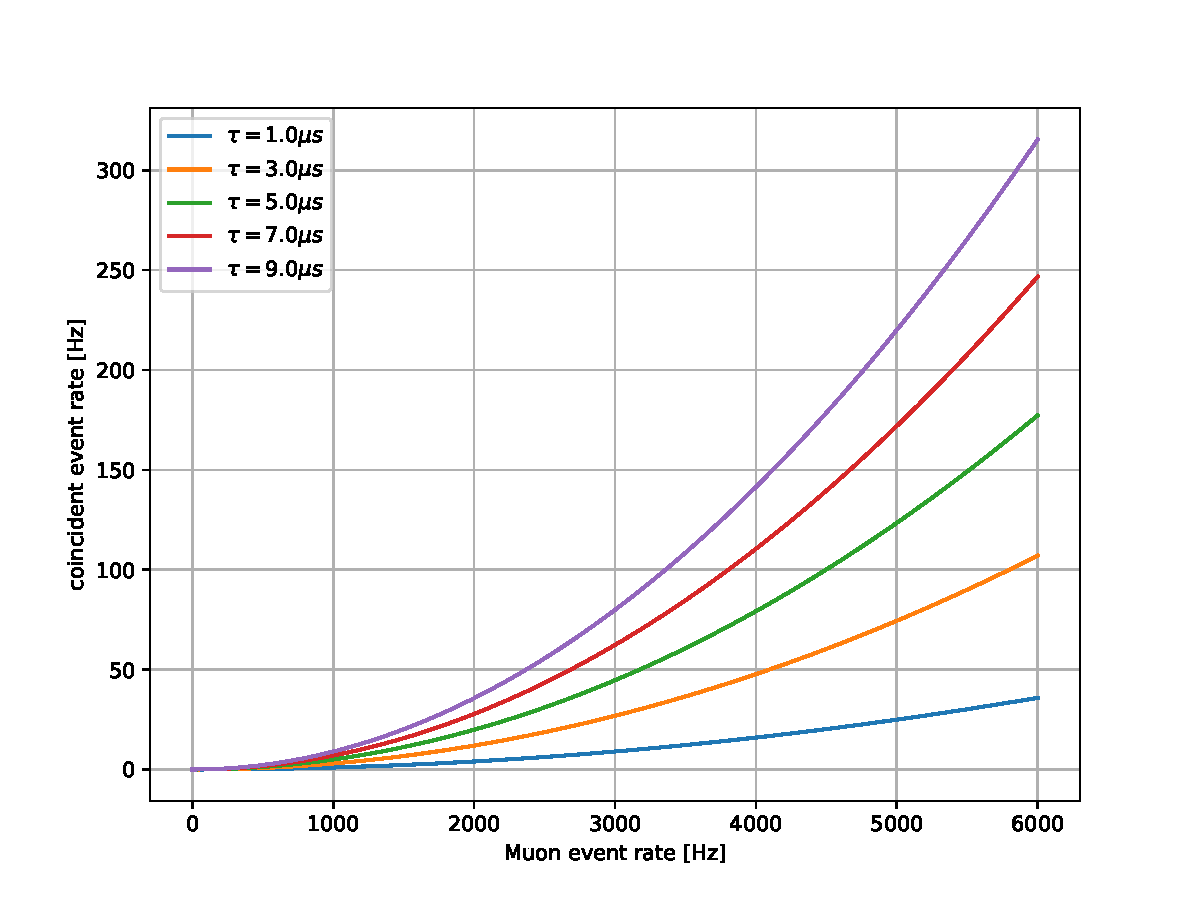
\includegraphics[width=0.7\textwidth]{Plots/coincidence_rate_poisson.pdf}
    \caption{A graph showing the relation between the muon event rate and the corresponding event rate assuming a poisson distributed muon event rate.}
    \label{fig:coin_rate_rate}
\end{figure}

In order to put this into a meaningful context, a relation of the muon event rate and their corresponding energy is extracted from a monte carlo simulation.
With this data describing a step function $rate(energy)$, equation~\ref{eq:multi_rate} can be used to visualize the relation between the muon energy and their 
corresponding rate of coincident events. Equivalent calculations are made on a zenith angle spectrum, for which the data is extracted from the same set of monte 
carlo data. Both of these distributions, along with the corresponding intervals, in which the coincidence probability exceeds \SI{0.1}{\percent}, are shown in 
figure~\ref{fig:coin_rate_combined}.

\begin{figure}[ht]
    \centering
    \begin{subfigure}[b]{\textwidth}
        \centering
        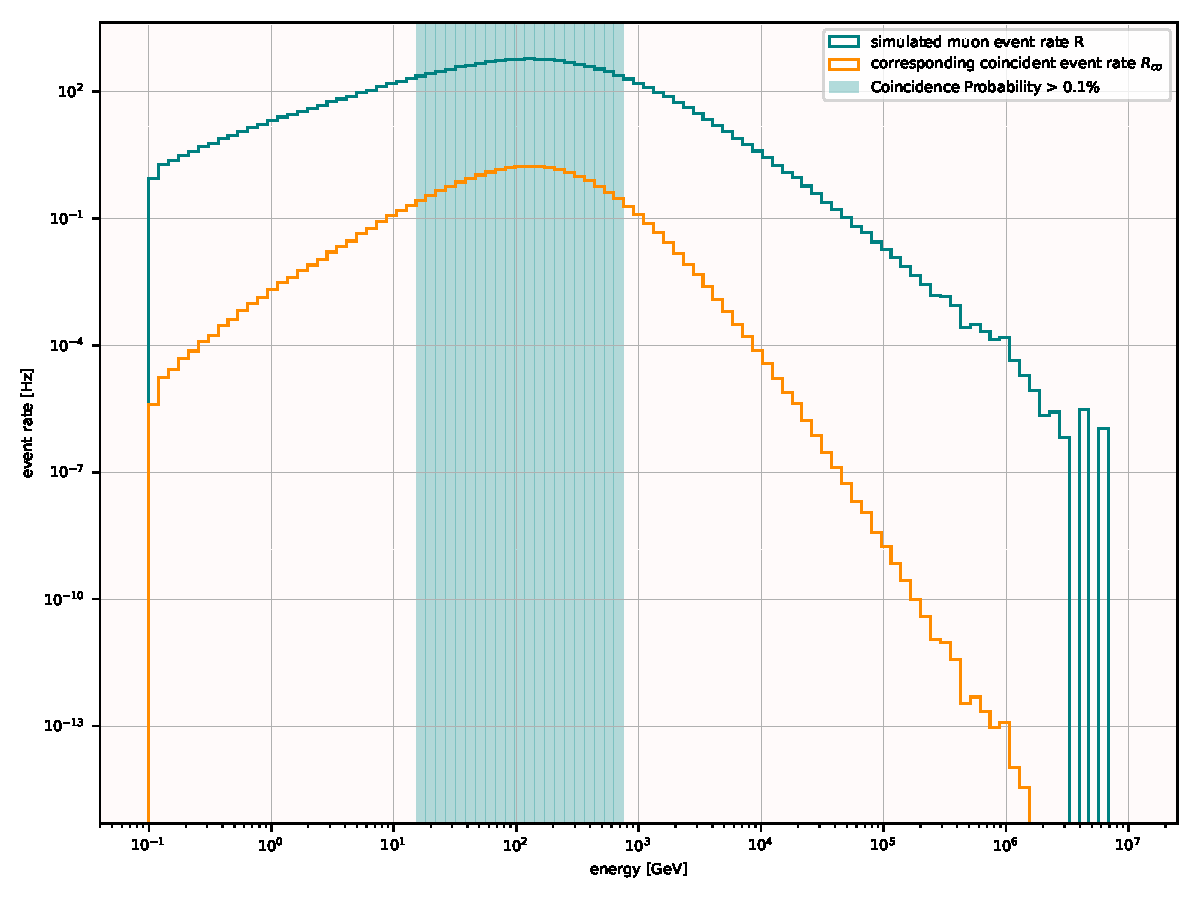
\includegraphics[width=0.7\textwidth]{Plots/coincidence_rate_energy.pdf}
    \end{subfigure}
    \vspace{1em} % Optional vertical space between the plots
    \begin{subfigure}[b]{\textwidth}
        \centering
        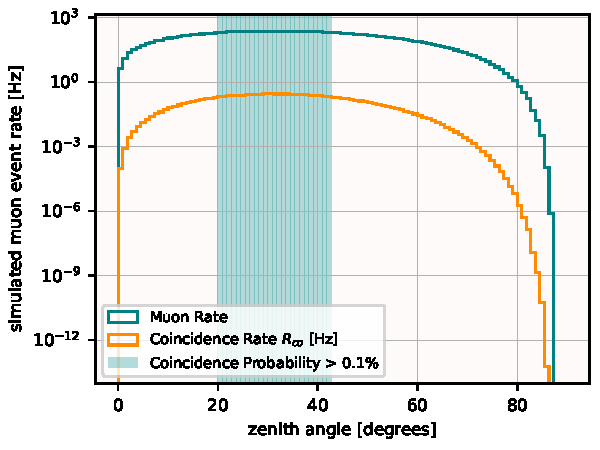
\includegraphics[width=0.7\textwidth]{Plots/coincidence_rate_zenith.pdf}
    \end{subfigure}
    \caption{Comparisons of the muon event rate and corresponding coincident event rate on energy and zenith angle spectra.}
    \label{fig:coin_rate_combined}
\end{figure}


Both histograms only show the theoretical coincidence event rate for a fixed trigger window $\tau$. However, diffrent triggers have diffrent readout windows, which 
can significantly change the probability of a coincident event. Treating the readout window as a variable, the coincident event probabilities can be visualized in 
a heat map to get a look at the effects of differing readout windows, as shown in figure~\ref{fig:heatmaps_combined}.

\begin{figure}[ht]
    \centering
    \begin{subfigure}[b]{\textwidth}
        \centering
        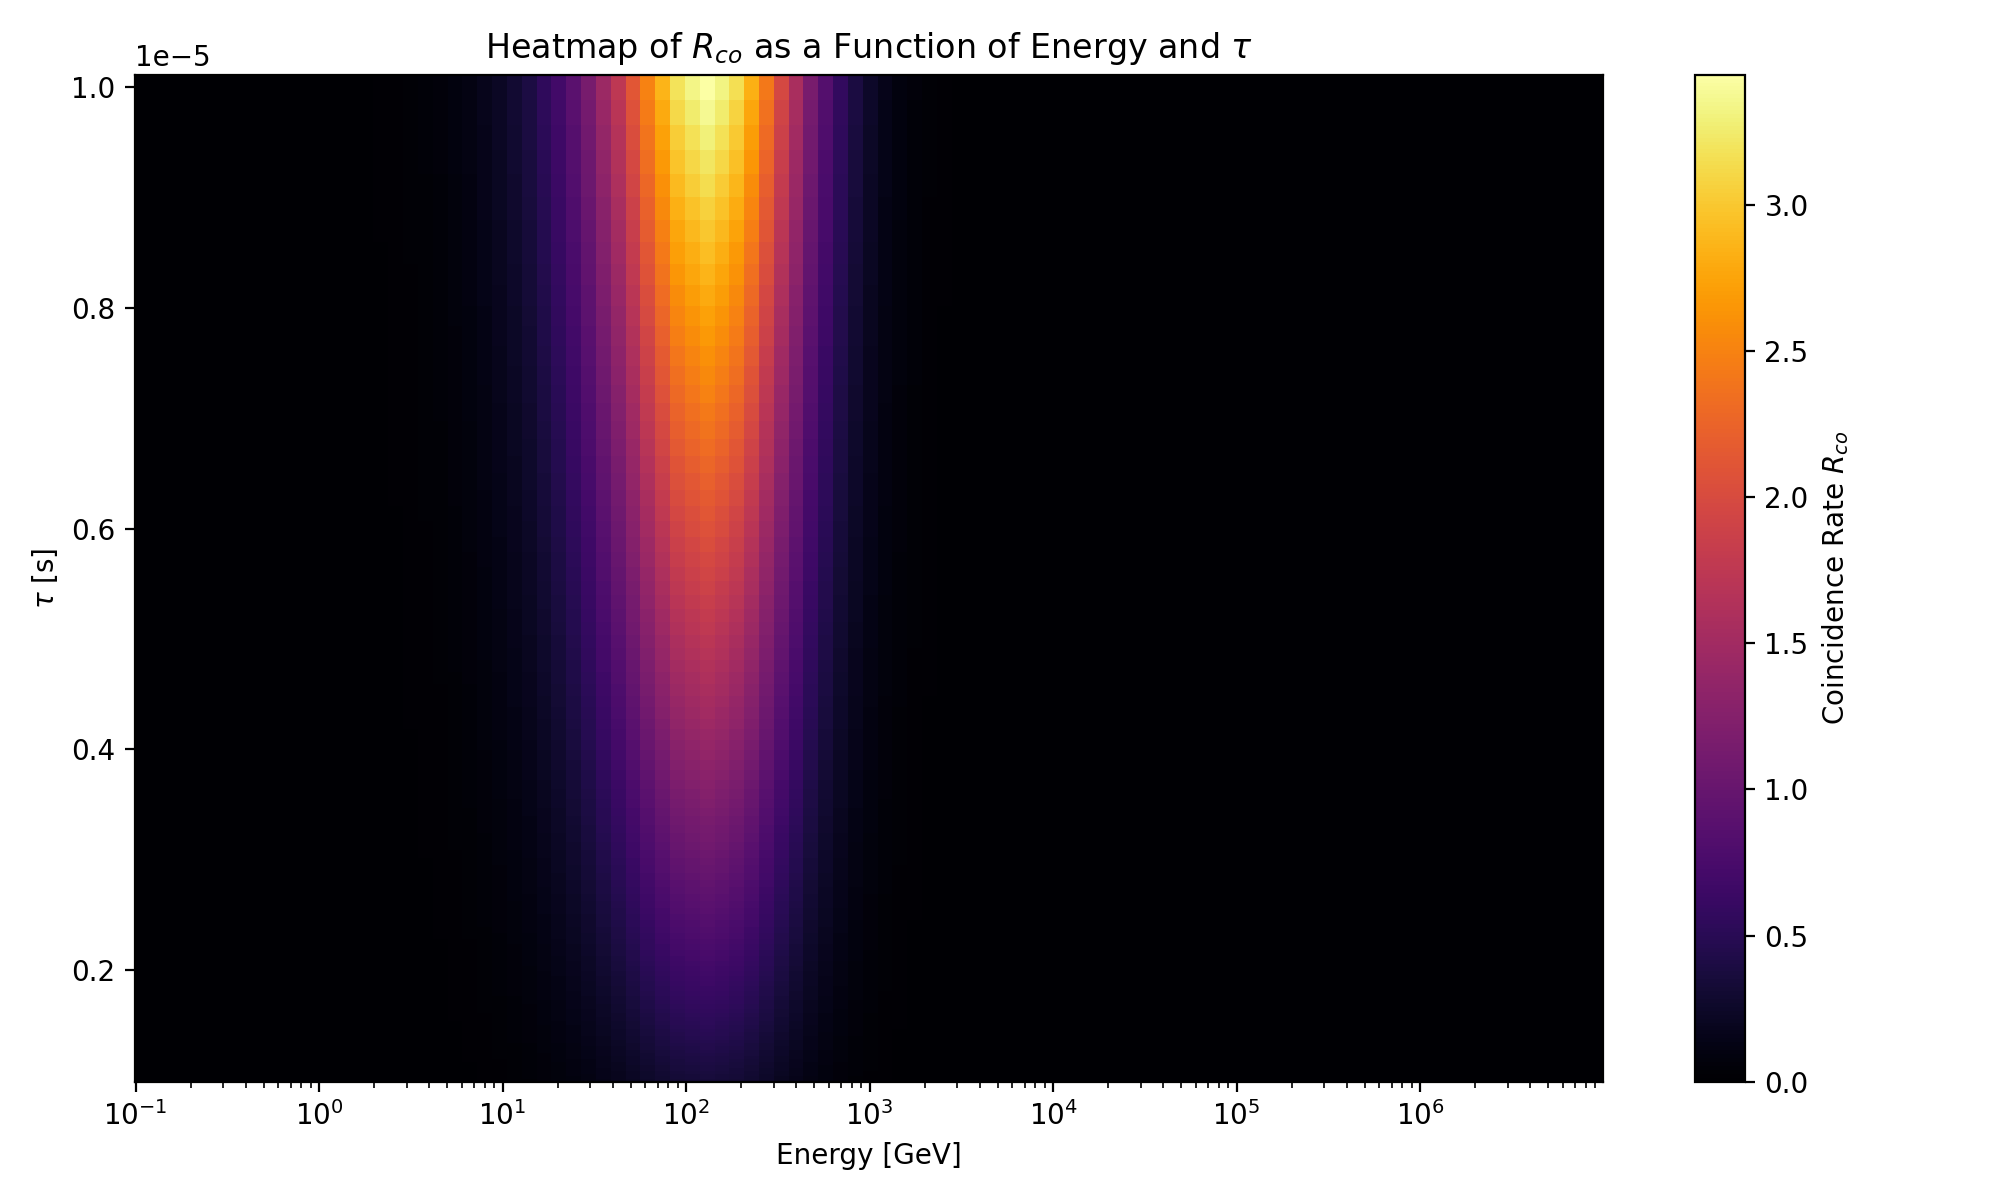
\includegraphics[width=0.7\textwidth]{Plots/heatmap_energy.png}
    \end{subfigure}
    \vspace{1em} % Optional vertical space between the plots
    \begin{subfigure}[b]{\textwidth}
        \centering
        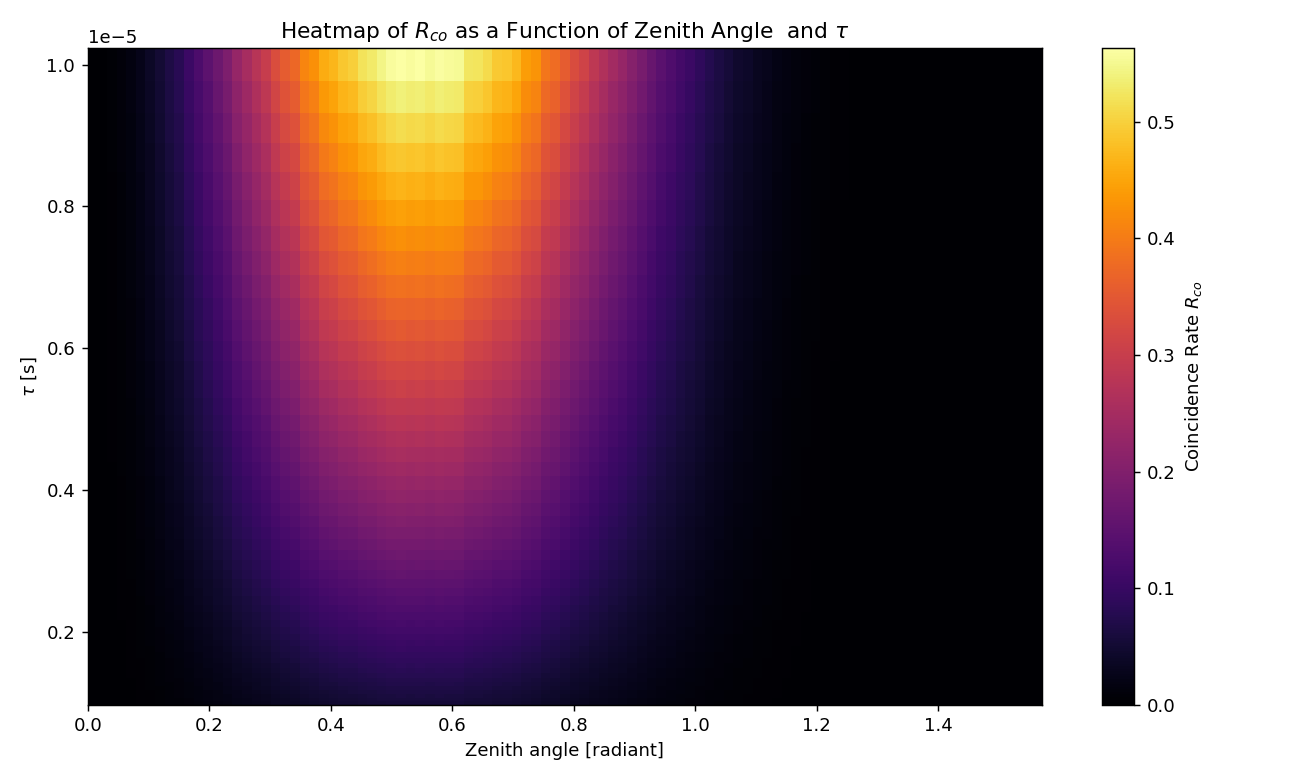
\includegraphics[width=0.7\textwidth]{Plots/heatmap_zenith.png}
    \end{subfigure}
    \caption{Prototypes of the heatmaps for energy and zenith angle spectra.}
    \label{fig:heatmaps_combined}
\end{figure}

\section{Analysis of the Fixed Rate Trigger}

As mentioned in section~\ref{sec:daq}, the FRT has a comparatively large readout window of \SI{10}{ms}. The result of this is that one \textit{event} contains 
a substantial amount of DOM hits. Since the average muon rate in IceCube is around \num{2200}\unit{Hz}, there is a significant likelihood, that any \textit{event}
contains physically significant signals. Other than muon events, there might be neutrino events as well as other possible atmospheric or astrophysical signals 
being measured in a given readout window of the FRT. However, a major fraction of the signals detected by the FRT is expected to be noise. 
(wie gibt man den Datensatz an, gibt es da einen standart?). The subsequent analysis is an attempt to extract knowledge about the composition of the signals 
measured by FRT and to possibly use them to better understand coincident events in IceCube.\\

The first step breaking down the FRT's data is to inspect the kind of signals detected in a singular DOM hit. In accordance with the description of 
\textit{subevents} in \ref{sec:daq}, a python script is used to filter out the corresponding signals (detaillierter~?). Depicted in 
figure~\ref{fig:frt_mu_sub_comp_1} is a comparison of the unfiltered and filtered signals detected over the course of \num{5035} \textit{events}. Most notably, 
the two distributions show a 
general similarity between them. As expected, there are substantially more unfiltered signals than filtered signals, showing that there are infact signals 
being filtered. The expectation would be to see a clear shift towards higher 
charge values in distribution of filtered signals, based on the idea that signals which stem from astrophysical or atmospheric sources would carry higher energy 
than noise signals. The observation does not quite match this expectation of clearly distinguished distributions. 

\begin{figure}[H]
    \centering
    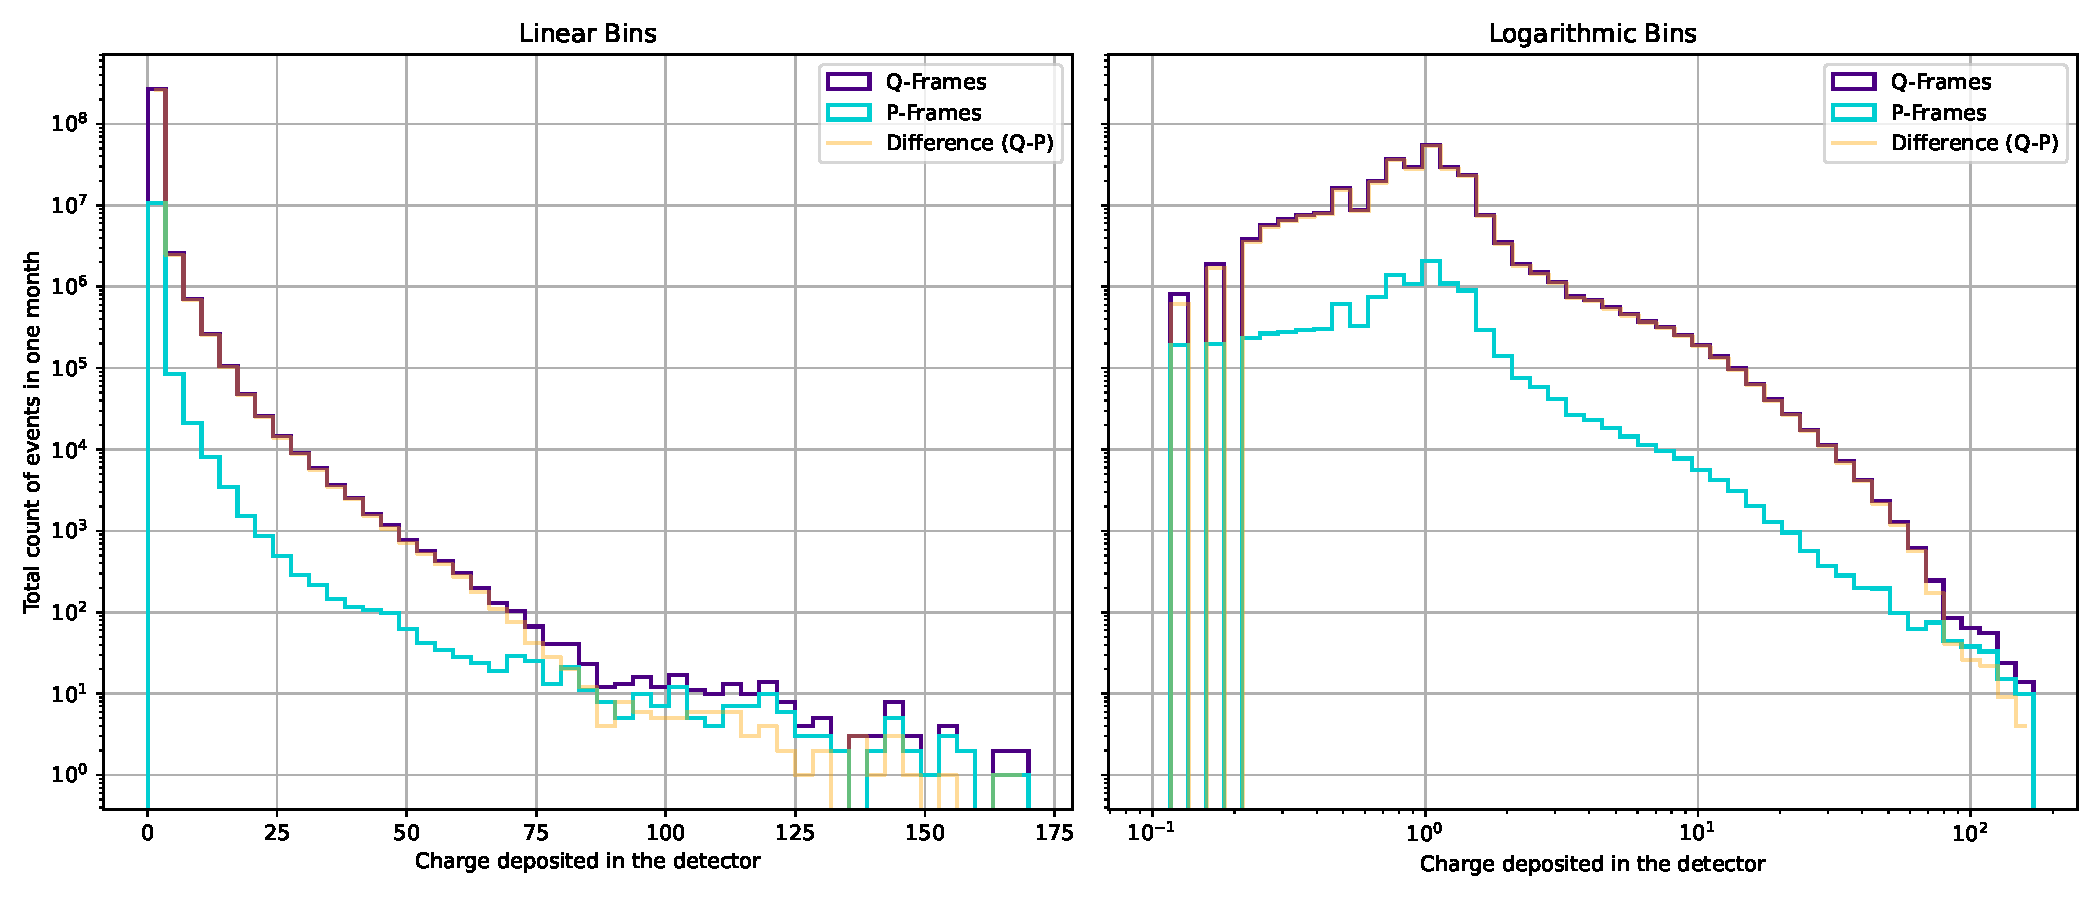
\includegraphics[width=\textwidth]{Plots/q_p_comp.pdf}
    \caption{A comparison between the counts of all Signals and physics signals.}
    \label{fig:frt_mu_sub_comp_1}
\end{figure}

To gather a deeper understanding of the signals measured and how they might be filtered, a comparison of mean charges for the individual DOMs is created. 
Figure~\ref{fig:mean_dom_charge_pq} shows the mean charge per DOM hit of every individual DOM over \num{5035} \textit{events}. 
The mean charges are quite evenly distributed throughout the DOMs, with the exeption of the DOM (61,13), which shows an unusually high mean charge of 
\num{5.08}~\unit(PE). Another notable characteristic of the filtered signals, although not easily visible, is the slightly higher mean charge around the 35th OM. 
%(values)
Other than that, there are no immediately visible anomalies in the general pattern of mean charges throughout the detector. 

\begin{figure}[H]
    \centering
    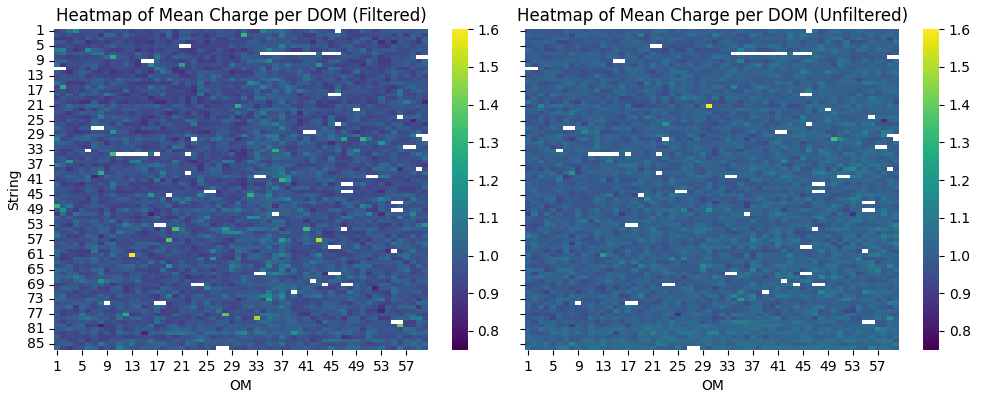
\includegraphics[width=\textwidth]{Plots/mean_charge_all_dom.png}
    \caption{The mean charge of every individual DOM for filtered and unfiltered signals.}
    \label{fig:mean_dom_charge_pq}
\end{figure}

While the analysis of mean charges over time allow for the possible detection of general anomalies or trends in the DOMs, it does not provide clear indicators for 
significant signals without additional information. When detecting a substantial signal, the expected behavior is a clear spike in the charge over function. 
Measuring these signals frequently might therefore have a visible impact on the standard deviation of the measured charge. The comparison of filtered and unfiltered 
signals regarding the mean charge values and their standard deviation is shown in figure~\ref{fig:mean_std_comp}.

\begin{figure}[H]
    \centering
    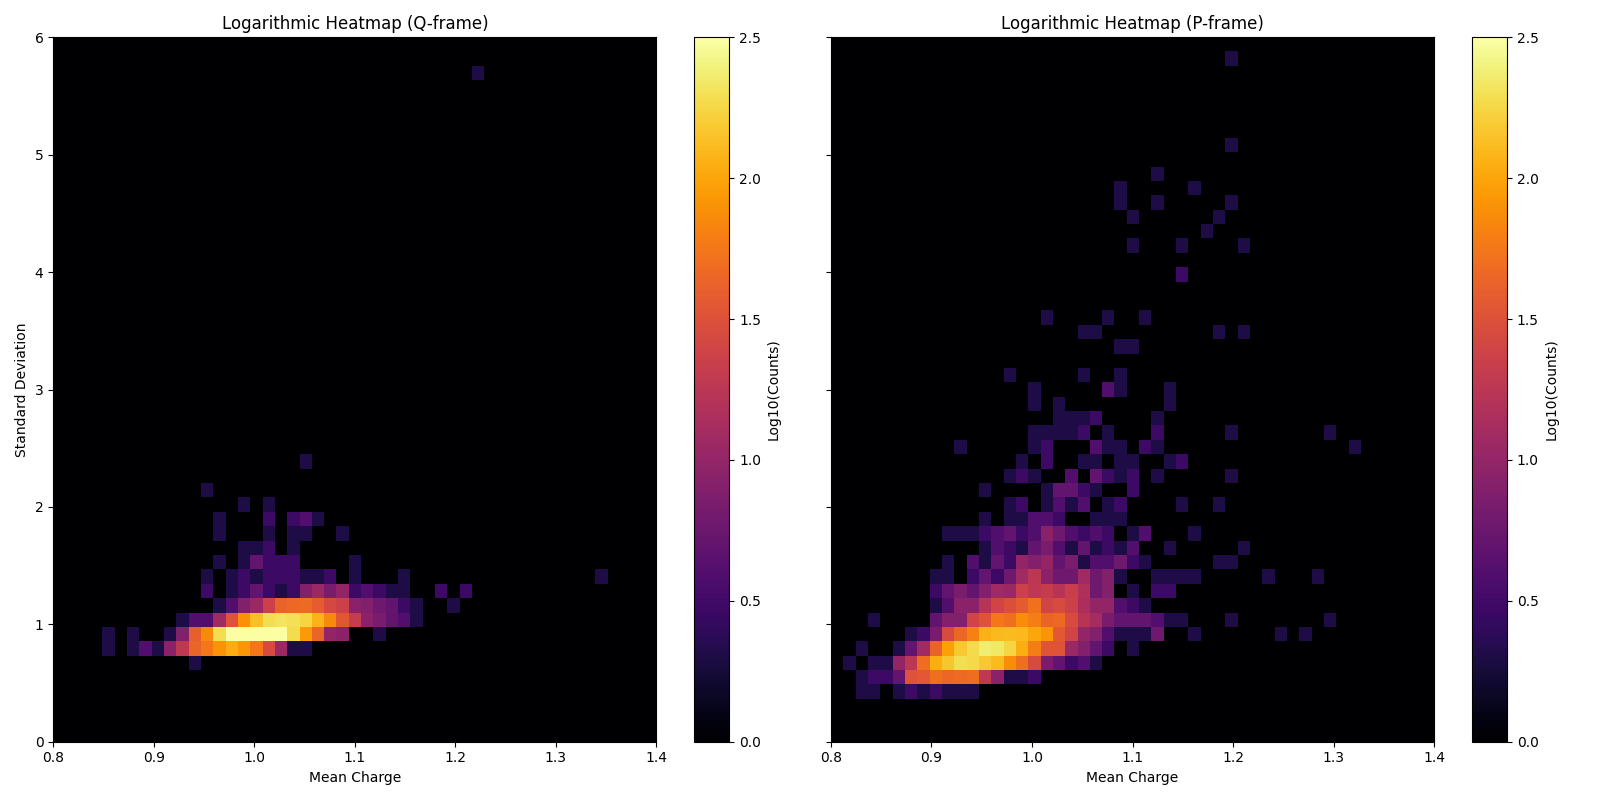
\includegraphics[width=0.9\textwidth]{Plots/mean_std_charge.png}
    \caption{A Comparison of the mean charge and standard deviation for filtered and unfiltered signals.}
    \label{fig:mean_std_comp}
\end{figure}

Clearly visible is the substantially larger spread of charges in the filtered signals. While the mean charges do not differ significantly from those of the 
unfiltered signals, there is a notable tendency towards larger deviation from the mean charge for the filtered signals. 
While this tendency suggests multiple measurements of high energy signals in those DOMs which show these high standard variations, the observation that the vast 
majority of filtered signals are clustered around a similar mean charge and standard deviation, as seen in figure~\ref{fig:mean_std_hist}, leads to the speculation 
that the filtered signals might still contain a considerable amount of noise.

\begin{figure}[H]
    \centering
    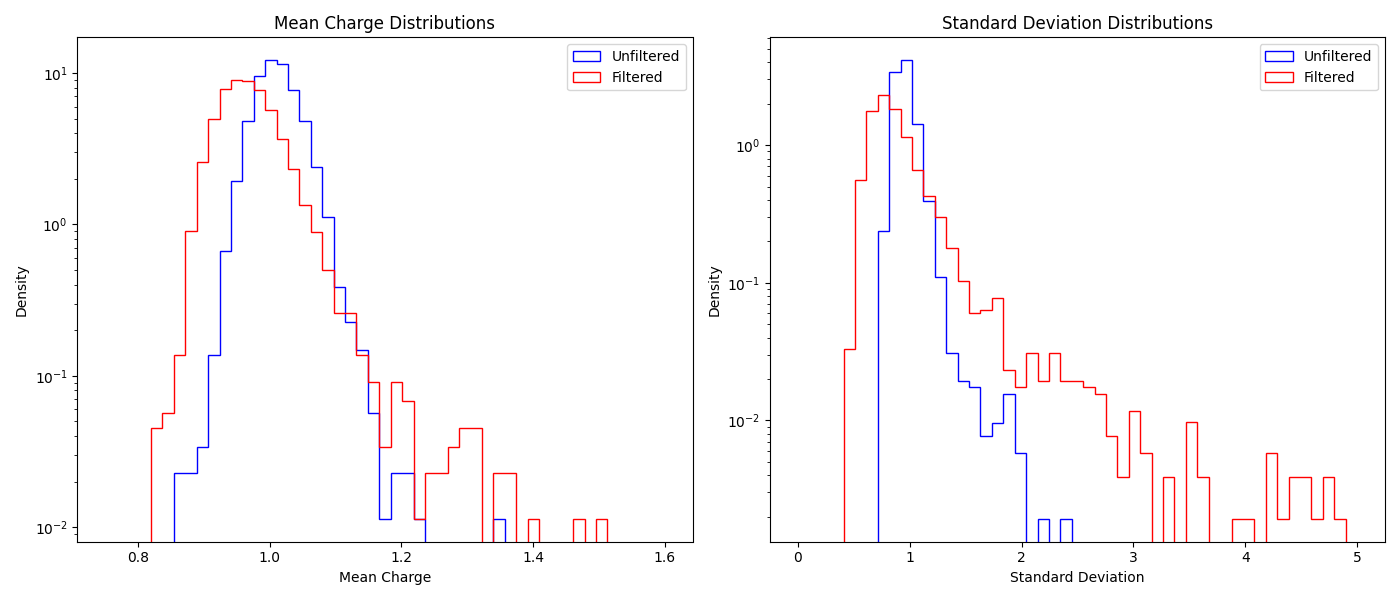
\includegraphics[width=0.9\textwidth]{Plots/qp_mean_std_comparison_histograms.png}
    \caption{An Individual Comparison of the mean charge and standard deviation.}
    \label{fig:mean_std_hist}
\end{figure}

Another interpretation could be, that the majority of signals of interest have infact comparatively low energies, leading to an average charge per DOM hit of 
just below \num{1}\unit{PE}. A disirable characteristic to observe would have been a certain charge threshold, below which none of the filtered signals 
would be observed. This would result in a strict condition that could be applied to certain triggers or other software. However, this is not the case. 

% further analysis:
% 1. charge over time p and q
% 2. charge over time in single events
% 3. filtermask with different plots
% 4. filter event candidates via simple algorithm -> clusters

Thus far, the signals detected by the FRT have been analyzed with a focus on individual DOM behavior. Another important property to examine is the charge per 
time function within singular events. Since one event accompasses a time window of \SI{10}{\milli\second}, a substantial amount of signals should be 
recorded for one event. This charge distribution over time for the entire detector is shown in figure~\ref{fig:charge_time_1}.

\begin{figure}[ht]
    \centering
    \begin{subfigure}[b]{\textwidth}
        \centering
        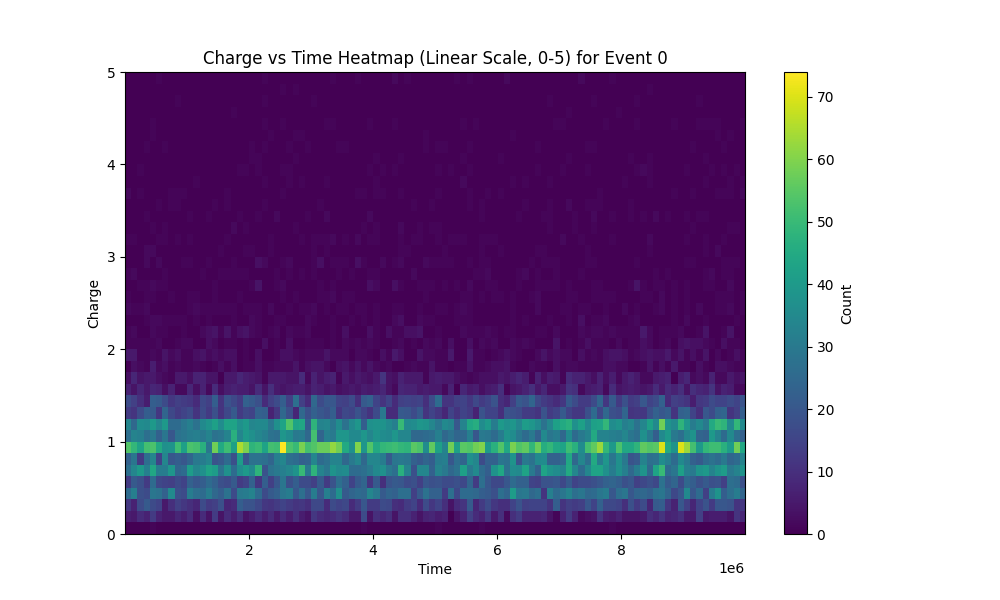
\includegraphics[width=0.7\textwidth]{Plots/charge_time_1_lin.png}
    \end{subfigure}
    \vspace{1em} % Optional vertical space between the plots
    \begin{subfigure}[b]{\textwidth}
        \centering
        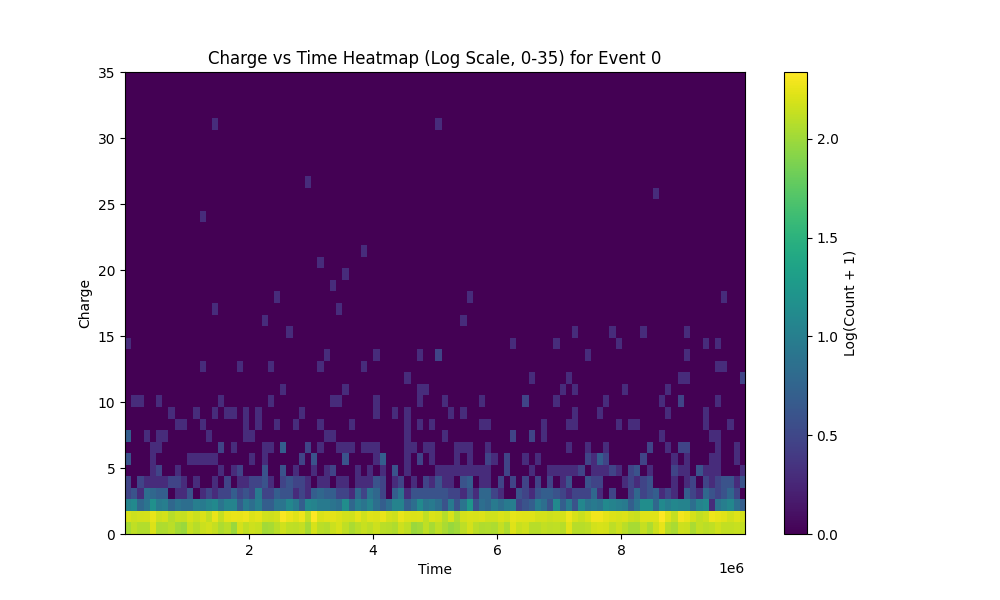
\includegraphics[width=0.7\textwidth]{Plots/charge_time_1_log.png}
    \end{subfigure}
    \caption{charge per time within one event (entire detector).}
    \label{fig:charge_time_1}
\end{figure}

Due to the long readout window of the FRT, the distribution of charge per time is visibly even during the event and does not differ significantly between 
individual events. This leads back to the inspection of the filtered signals. These signals are clustered in subevents, which should have significantly
more distinct features with regards to their corresponding charge over time measurements. From the previous analysis however, these filtered subevents 
have been shown to contain a substantial amount of signals with comparatively low charges. As a visual comparison, two subevents with comparatively high 
total charge are shown next to two average subevents. 

\begin{figure}[h!]
    \centering
    % First row
    \begin{subfigure}[t]{0.49\textwidth}
        \centering
        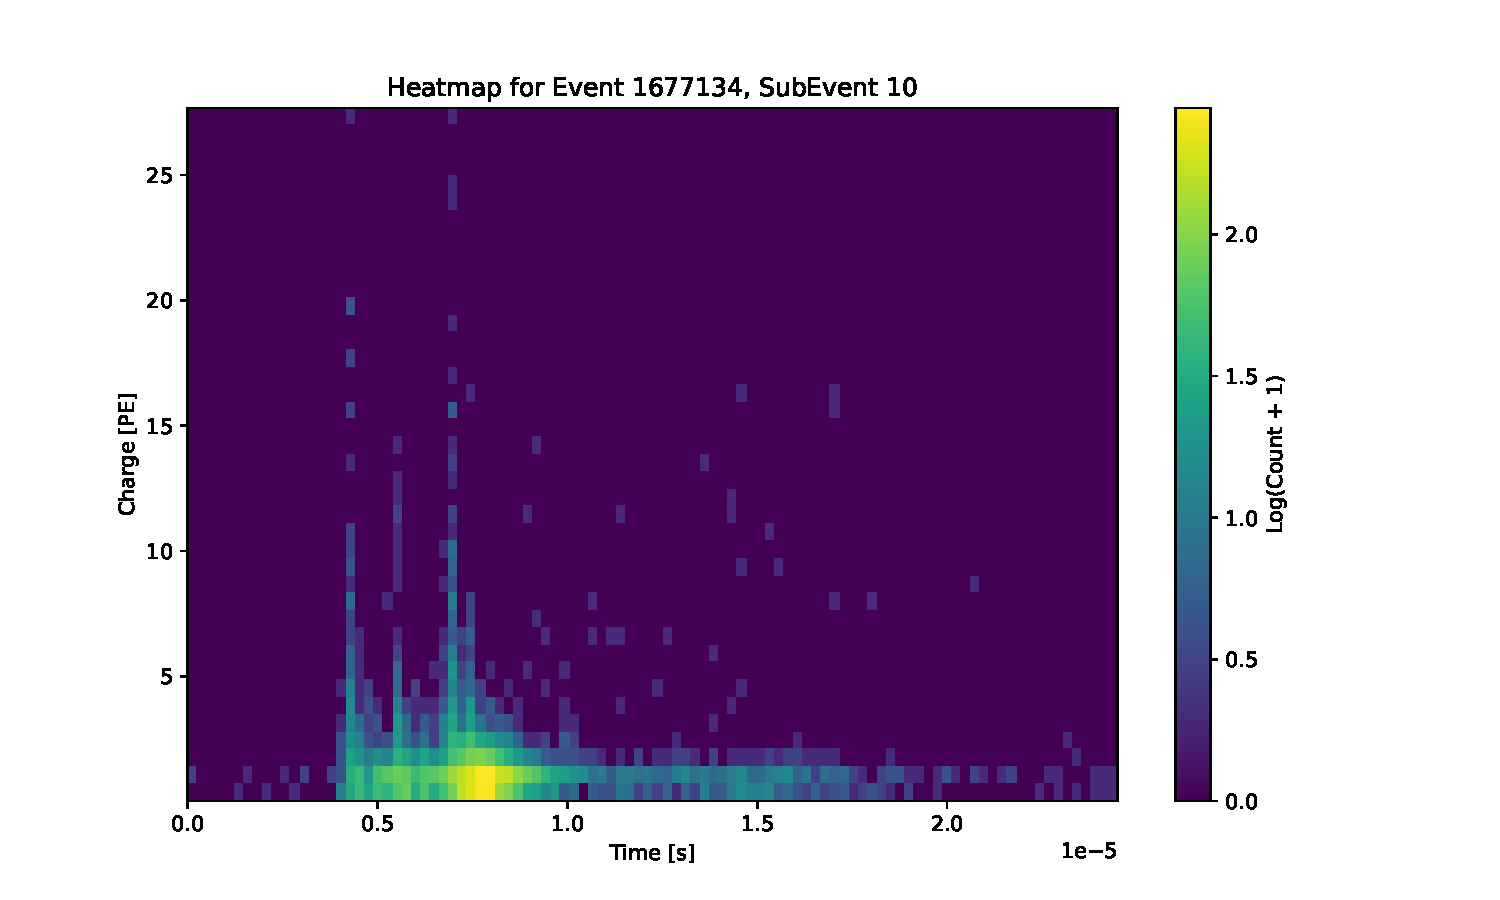
\includegraphics[width=\textwidth]{Plots/heatmap_subevent_triple_high.pdf}
        \caption{SubEvent 1: Description here.}
        \label{fig:subevent1}
    \end{subfigure}
    \hfill
    \begin{subfigure}[t]{0.49\textwidth}
        \centering
        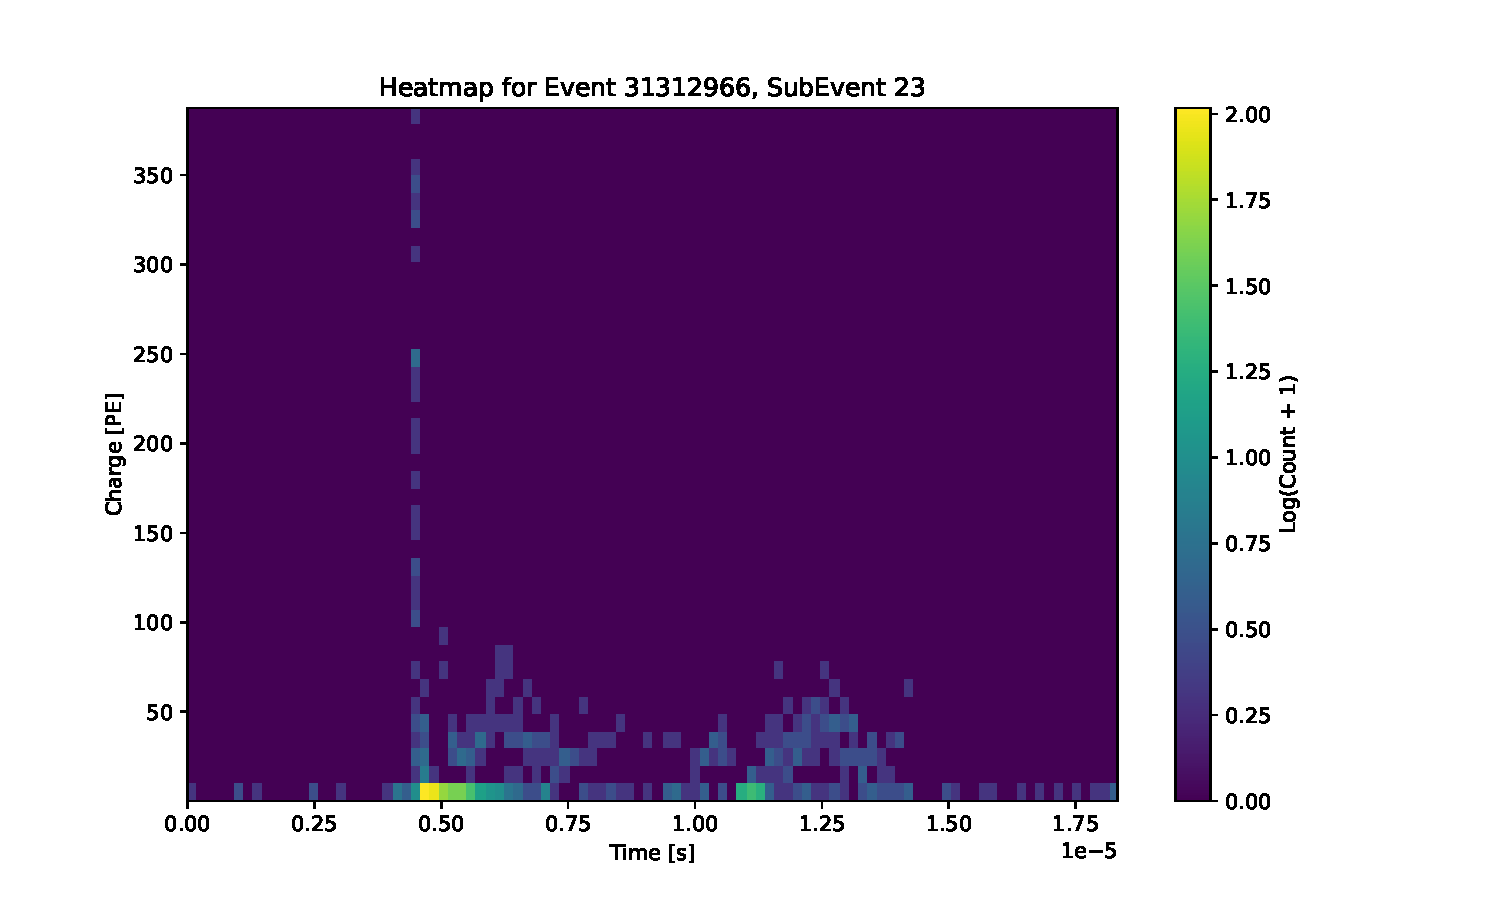
\includegraphics[width=\textwidth]{Plots/heatmap_subevent_double_high.pdf}
        \caption{SubEvent 2: Description here.}
        \label{fig:subevent2}
    \end{subfigure}
    
    % Second row
    \vspace{0.5cm} % Adjust vertical spacing as needed
    \begin{subfigure}[t]{0.49\textwidth}
        \centering
        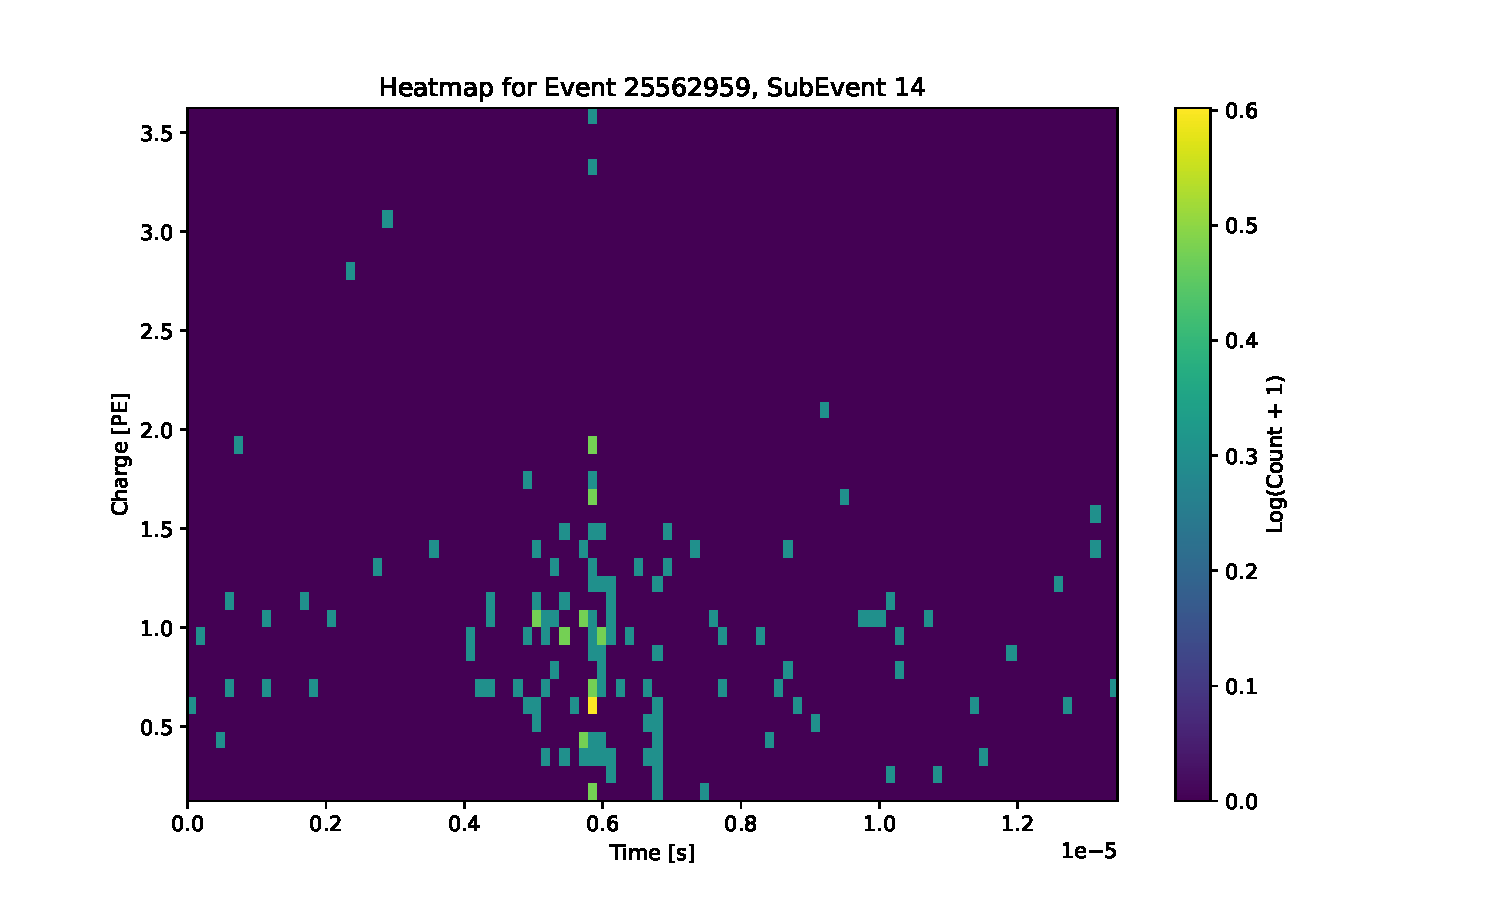
\includegraphics[width=\textwidth]{Plots/heatmap_subevent_random_1.pdf}
        \caption{SubEvent 3: Description here.}
        \label{fig:subevent3}
    \end{subfigure}
    \hfill
    \begin{subfigure}[t]{0.49\textwidth}
        \centering
        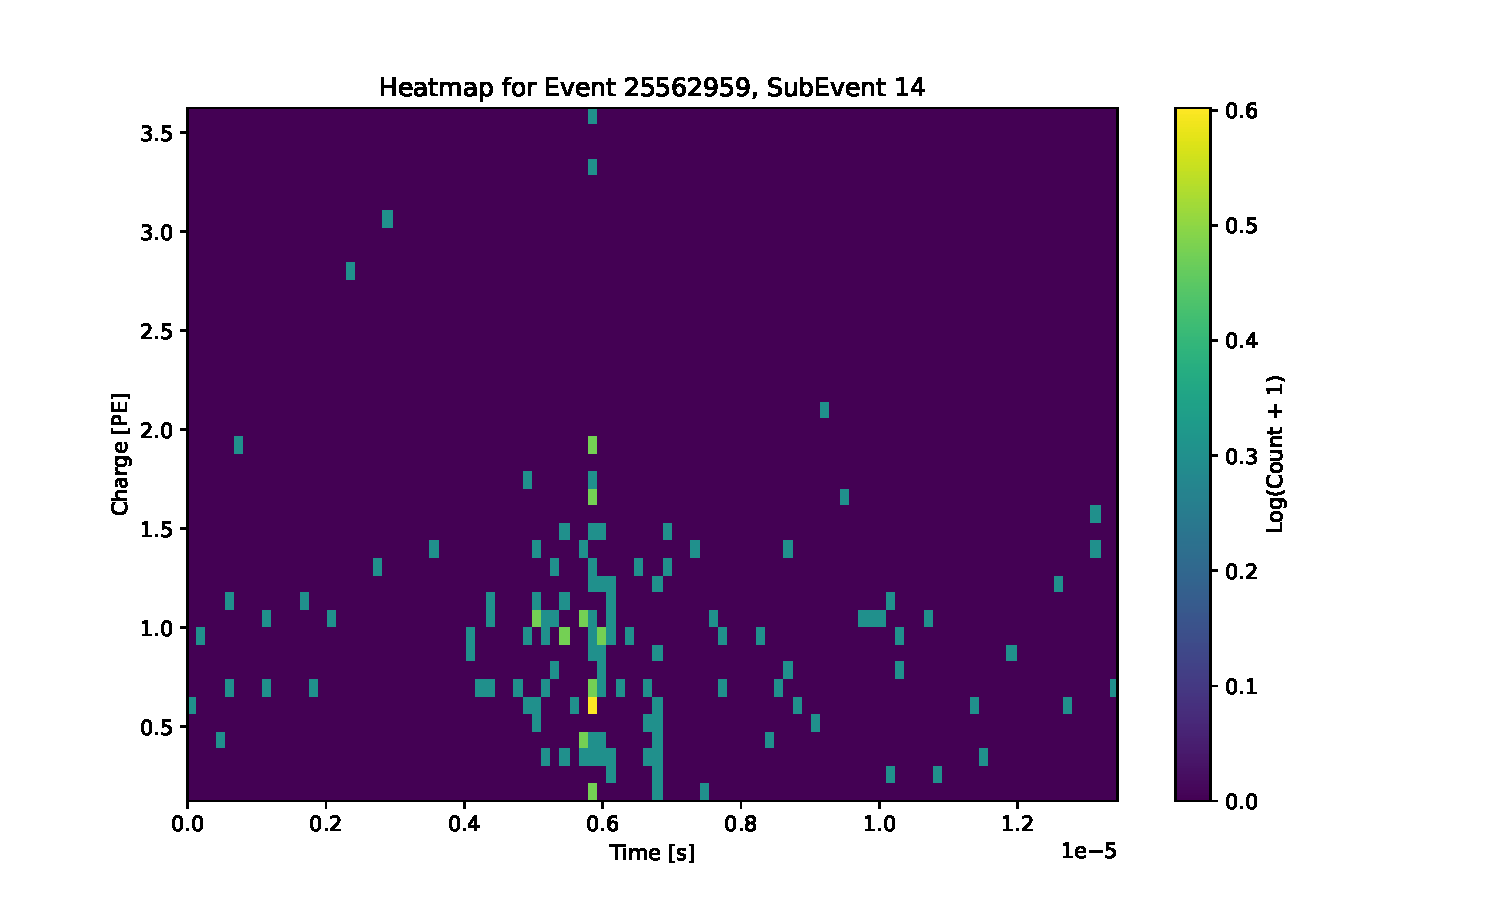
\includegraphics[width=\textwidth]{Plots/heatmap_subevent_random_1.pdf}
        \caption{SubEvent 4: Description here.}
        \label{fig:subevent4}
    \end{subfigure}

    % Main caption for the figure
    \caption{Comparison of heatmaps for four different SubEvents. }
    \label{fig:subevent_charge_time}
\end{figure}

While the visual difference between these subevents of vastly differing mean charge is immediately evident, a specificly interesting characteristic can be 
observed for the subevents 1 and 2. These subevents show multiple peaks of charge and signal count within their individual time frame. As these features
might be indicators for coincident events, these structures are analyzed in detail. 

There are a variety of possible approaches for identifying possible coincident event candidates. In the subsequent analysis, the python function $\text{find\_peaks}$ 
from 
the scipy library is used. Singular events are characterized by a combindation of the charge values, as well as the signal counts on a time scale within the time 
frame of a subevent. This time frame is divided into \num{100} equally spaced bins. For each bin, the sum of the charges ($Q_P$) measured within is calculated, 
as well as the total counts ($N_P$) within in the bin. These projections are combined into a weighted projection ($W_P$)

\begin{equation}
    W_P = \alpha\cdot Q_P +  \beta\cdot N_P\,
\end{equation}

where the weights \alpha and \beta are calculated via the equation

\begin{align}
    \alpha &= \frac{M_N + \sigma_N^2}{(M_C + \sigma_C^2) + (M_N + \sigma_N^2)} \\
    \beta &= 2\frac{M_C + \sigma_C^2}{(M_C + \sigma_C^2) + (M_N + \sigma_N^2)}
\end{align}


where $(M_C)$ and ($M_N$) represent the sums of the charge and count projections, respectively, and ($\sigma_C^2$) and ($\sigma_N^2$) denote their variances. 
These weights ensure that both the magnitude and variability of the projections are accounted for in the weighted projection. 

$W_P$ is then used as the function for which the $\text{find\_peaks}$ method is applied. This method takes multiple parameters, which were determined empirically 
based on a variety of subevent samples. These parameters are shown in table~\ref{tab:peak_parameters} along with their respective description.


\begin{table}[h!]
    \centering
    \begin{tabular}{|l|l|p{7cm}|}
    \hline
    \textbf{Parameter} & \textbf{Value} & \textbf{Description} \\ \hline
    Prominence & 5 & The minimum vertical distance a peak must stand out relative to its neighboring valleys. This ensures that only significant peaks are detected. \\ \hline
    Height & Dynamic (\(5\%\) baseline + \(1.5 \cdot \sigma\)) & The minimum value a peak must reach to be considered valid. This threshold is calculated dynamically based on the signal's baseline noise (5th percentile) and its standard deviation (\(\sigma\)). \\ \hline
    Distance & 4 bins & The minimum number of bins required between consecutive peaks to ensure they are sufficiently separated and not falsely grouped. \\ \hline
    \end{tabular}
    \caption{Final parameters used for peak detection in the weighted projection of charge and count data.}
    \label{tab:peak_parameters}
\end{table}


The workings of this method are visualized for an example subevent in figure~\ref{fig:find_peaks}

\begin{figure}[ht]
    \centering
    \begin{subfigure}[b]{\textwidth}
        \centering
        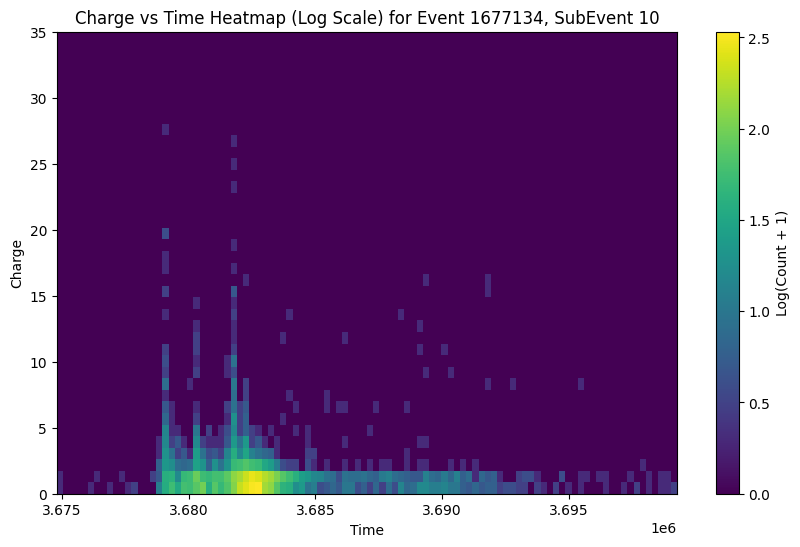
\includegraphics[width=0.7\textwidth]{Plots/peak_heat_1.pdf.png}
    \end{subfigure}
    \vspace{1em} % Optional vertical space between the plots
    \begin{subfigure}[b]{\textwidth}
        \centering
        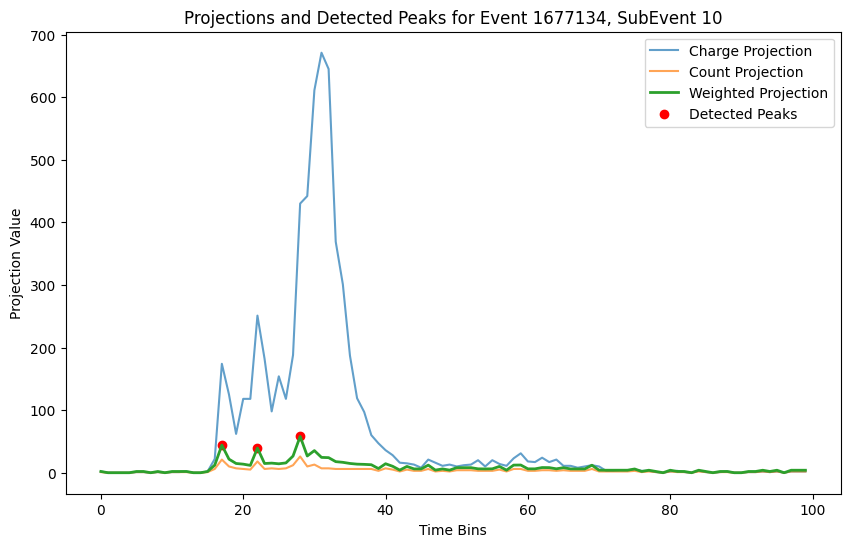
\includegraphics[width=0.7\textwidth]{Plots/peak_plot_1.png}
    \end{subfigure}
    \caption{caption}
    \label{fig:find_peaks}
\end{figure}

While this method seems to be working decently well for subevents with large enough charges, it struggles with those subevents that lack distinctly defined 
features. With the current set of parameters, the following results are concluded:

\begin{align}
    total subevents &= 137342 \\
    \frac{N(multiple peaks)}{N(any peaks)} &= 0.54 \\
    \frac{N(any peaks)}{N(total)} &= 0.85
\end{align}

The evaluation of these results is discussed in the subsequent chapter~\ref{chap:discussion}











\chapter{Discussion of Results}\label{chap:discussion}

\section{Theoretical Calculations}
The calculations of the theoretical coincident muon event rate in section~\ref{sec:muon_coincidence} provide a simple framework for estimating 
coincident event probabilities under varying trigger windows. As seen in figure~\ref{fig:coin_rate_combined}, the theoretical coincidence probability 
exceeds \SI{1}{\percent} for a readout window of \SI{5}{\micro\second} for significant intervals of both the energy- and the zenith angle spectrum. 
Even if this probability is subject to further variables, as it most likely is, it appears that the magnitude of coincident events is at least 
significant enough to consider for precise analyses. As the analysis here is only based on Monte Carlo simulations, similar evaluations based on 
experimental data could be interesting. Also, further variables could be taken into account.
Based on where in the detector two or more events are detected around the same time, the spatial and geometric conditions for certain triggers could have 
an impact on the likelihood of a coincident getting detected as such. 

\section{Fixed Rate Trigger}
Analyzing the FRT data in detail serves as an interesting insight into the unfiltered patterns of detected signals in IceCube. The comparison of filtered 
and unfiltered signals revealed, that filtering by physically relevant signals does not justify any cutoff at low charges, as shown in figure~\ref{fig:frt_mu_sub_comp_1}.
While this reality created significant challenges for the subsequent analyses, it is a valuable finding and should be analyzed further. 
The main challenge arising from the lack of a clear distinction between signals and possible noise was, that characterizing possible event or coincident event candidates 
proved difficult. As a result, a number of the analyses created for the FRT data were left with no concrete results. 
However, some interesting features were visible when analyzing the charge over time functions for different subevents, as shown in figure~\ref{fig:high_low_comp}.
This led to the attempt of characterizing possible coincident events. This attempt did not yield the desired level of success. As the features of coincident events 
are highly complex, the relatively simple approach of finding peaks in a projection of charge and frequency could be considered an oversimplification.
Still, inspecting the charges and counts of signals in the subevents as a function of time might be a valuable approach to finding coincident events, when combined
with different methods to search for clusters. Machine learning algorithms could be used for more a more complex search for distinguishing characteristics.

\section{Conclusion}
While the unsatisfactory lack of concrete results is undeniable, valuable insights were found on the FRT, which would not be accessible by analyzing any other 
datasets available for IceCube. Further evaluation and the use of machine learning algorithms could possibly lead to more concrete results in the future.

\appendix
% Hier beginnt der Anhang, nummeriert in lateinischen Buchstaben
\chapter{Appendix}

The analyses utilized the following Python libraries:

\begin{itemize}
    \item \textbf{NumPy}: For numerical computations and array operations.
    \item \textbf{SciPy}: For scientific computing and statistical analysis.
    \item \textbf{Matplotlib}: For data visualization.
    \item \textbf{Seaborn}: For statistical data visualization with enhanced aesthetics.
    \item \textbf{Pandas}: For data manipulation and analysis.
    \item \textbf{h5py}: For reading and writing HDF5 files.
\end{itemize}


\backmatter
\printbibliography

\cleardoublepage
% From https://www.tu-dortmund.de/studierende/im-studium/pruefungsangelegenheiten/allgemeine-vordrucke/
\includepdf{content/Eidesstattliche_Versicherung.pdf}

\end{document}
